\section{System-level modeling}
\label{sec:esd-modeling}

% Simulations are a key tool
Among all investigations and analysis methods, simulations are extremely important for understanding the impact of \gls{esd}s on integrated circuits.
Physical access to nets is extremely difficult in the actual chip
In simulation, any net can be instantly probed and its waveform displayed.

% But require a lot of preliminary effort
However, \gls{esd} simulations are far from trivial
For operating ESD, need electrical device models that work in normal operating conditions and in electrostatic domain of fast transients, highly non-linear and varying signals.
To build trust on the simulation results, models must be validated against measurement data, and in many different test conditions.

% Hierarchical level
Electronic systems are by nature hierarchical things
Large scale devices such as test generators impact small scale devices like integrated circuits, themselves composed on transistors and other electron devices.
For \gls{esd}, the question of the appropriate scale for performing the modelling is raised.
Compromise between the accuracy of models, the amount of effort and time for performing the modelling, simulation time
Accuracy at transistor-level is hardly possible, and is not necessarily required.
Different methods are probably required for different scale.

% Which level is targeted here
Focus in the first time on the system level.
Is considered a system any macro-scale device, such as an \gls{esd} generator or a lab equipment like a DC supply.
In this chapter, a methodology for building electrical models of systems and electrical setups is proposed.
Some presented concepts also apply at the board level, for quick modelling of \gls{pcb} metal tracks.

% Main concept
A modular approach is adopted.
Electronic systems and test setups are very often composed of a limited set of standard and common devices.
Equipments are made for example of DC sources, discrete passive devices, relays.
Equipments are connected together with the use of wires, twisted wire pairs, coaxial cables, etc.
The goal is to build a library of those discrete devices.
Each model of the library is qualified independently with measurements, which is easy to accomplish because the complexity is low and measurements can be easily acquired.
Later on, the architecture or the electrical circuit of a system serves as a blueprint to connect \gls{esd} models from the library together in order to obtain a complete and accurate model of the system.

% Limits in voltage/time
%TODO: Mouais, a revoir
The methodology applies for models with the aim to perform transient simulations from normal operating timescale down the nanosecond timescale, and with voltage and current levels well above normal operating conditions.

% Structure of the next section ?
Discrete devices
Application

\subsection{Lossless transmission line}

\gls{esd} events generally last a few hundred nanoseconds.

Any element that introduces a delay in the same order of magnitude (down to the nanosecond) can impact the waveforms.
Delays and propagation phenomena in general can obviously offset a waveform in time,
but also cause ringing oscillations with a period directly proportionnal to the delay.

Delays can be generated by cables and metal tracks, such as coaxial cables, twisted wires, wires over ground \gls{pcb} traces and so on.

Most cables and PCB traces, although of very different construction, usually behave as lossless transmission lines and can be modeled as such.

A transmission line is defined by two key parameters, a \gls{Zc} and a propagation delay.


For a purely lossless transmission line, the characteristic impedance is purely real.
In practice, truly lossless cables do not exist.
However, most coaxial cables exihibit very low losses below frequencies of a couple GHz, which is sufficient during ESD simulations to consider them lossless.

% Distributed model
Physically, a transmission line is a distributed capacitance an inductance.
It can be modeled in a discrete manner, as a sum of unitary RLC elements.
The value for this unit element can be computed trivially from the characteristic impedance \gls{Zc}.

\begin{figure}[!h]
  \centering
  \includegraphics[width=0.3\textwidth]{src/1/figures/distributed_line_model.pdf}
  \caption{Electrical distributed model of a lossless transmission line}
  \label{fig:dis-line-model}
\end{figure}

EQUATION RLC vs Zc

A single element generates a delay DT, much smaller than the delay of the cable.
To model the entire cable, many instances of this element are connected in series.
There is a tradoff to make between the delay of the unit element and the total amount of unit elements required to model the cable.

A small delay makes the cable model more accurate, however, more elements are required for the total cable, which results in longer simulation times.
On the other hand, a larger delay will limit the accuracy of the simulation by reducing the bandwidth of the model, which is not desirable either.

The main advantage for the distributed model is its ability to support lossy transmission lines (to check if this is true for a TL that has variable losses at low freqs).

The main disavantage is that it does not scales well with longer delays.
To keep the same bandwidth with a longer cable, the only solution is to increase the element count, resulting in longer simulation time.

% Behavioral model
A behavioral model can describe efficiently and with great accuracy the behavior of most lossless transmission lines.

The electrical model is constituted of two voltage-controlled voltage sources and two resistors.
Compared to the classic RLC distributed model, the behavioral model has infinite bandwith, and constant complexity (compared to RLC where the amount of elements increases with the required bandwidth).

\begin{figure}[!h]
  \centering
  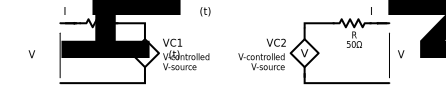
\includegraphics[width=0.3\textwidth]{src/1/figures/behavioral_line_model.pdf}
  \caption{Electrical behavioral model of a lossless transmission line}
  \label{fig:beh-line-model}
\end{figure}

EQUATIONS

The equations illustrate relations between incident and reflected waves, and voltage and current ratio.

Implementation in VHDL-AMS

%TODO: Code

% Conclusion

To determine which model performs best, a few simulations are compared.
The test setup consist of a square pulse voltage source, with a risetime of 1 ps, a transmission line, and an unmatched termination at 25 ohms.

The RLC model with different settings is compared to the behavioral model.

cable 10ns, 50ns ?

- Config accurate
- Config fast
- Config lossy ?

Overall, the behavioral model outperforms the distributed model.
It is much more accurate (because not inherently limited in bandwith) and extremely fast to simulate.

The main reason for using the distributed model is to take losses into account, which is rather rare in practice.

\subsection{Passive devices}

Non linear behavior in high-regime and high-frequency conditions \cite{capa-esd-cz}.

%TODO
For frequencies/bandwidth higher than the MHz, frequency behavior of  passive devices starts show up.
A simple rule of thumb for linking bandwidth (frequency domain) and signal rise time (time domain) is given by the following equation:

BW = 0.35 / risetime

For nanosecond risetimes (usual value for TLPs), the occupied bandwidth is over 350 MHz, well beyond the 1MHz limit.
In theory, with such fast risetimes, passive devices should all have a frequency-dependant model in order to well reproduce spikes and peaks in the simulations.

However, in practice, it was found that only devices directly in parallel of measurement probes or IC inputs needed a frequency dependant model.
This is especially true for decoupling capacitors, which usually have both of these two properties.
HF models for inductors, resistors and capacitors are given Fig. \ref{fig:rlc-esd-models}.

\begin{figure}[!h]
  \centering
  \includegraphics[width=0.3\textwidth]{src/1/figures/rlc_esd_models.pdf}
  \caption{High-frequency (a few GHz) models for resistor, capacitor and inductor}
  \label{fig:rlc-esd-models}
\end{figure}

Those HF models can be very quickly and easily parameterized.
Values to use can be extracted with an impedance meter capable of measuring impedances to at least 100 MHz.

\begin{figure}[!h]
  \centering
  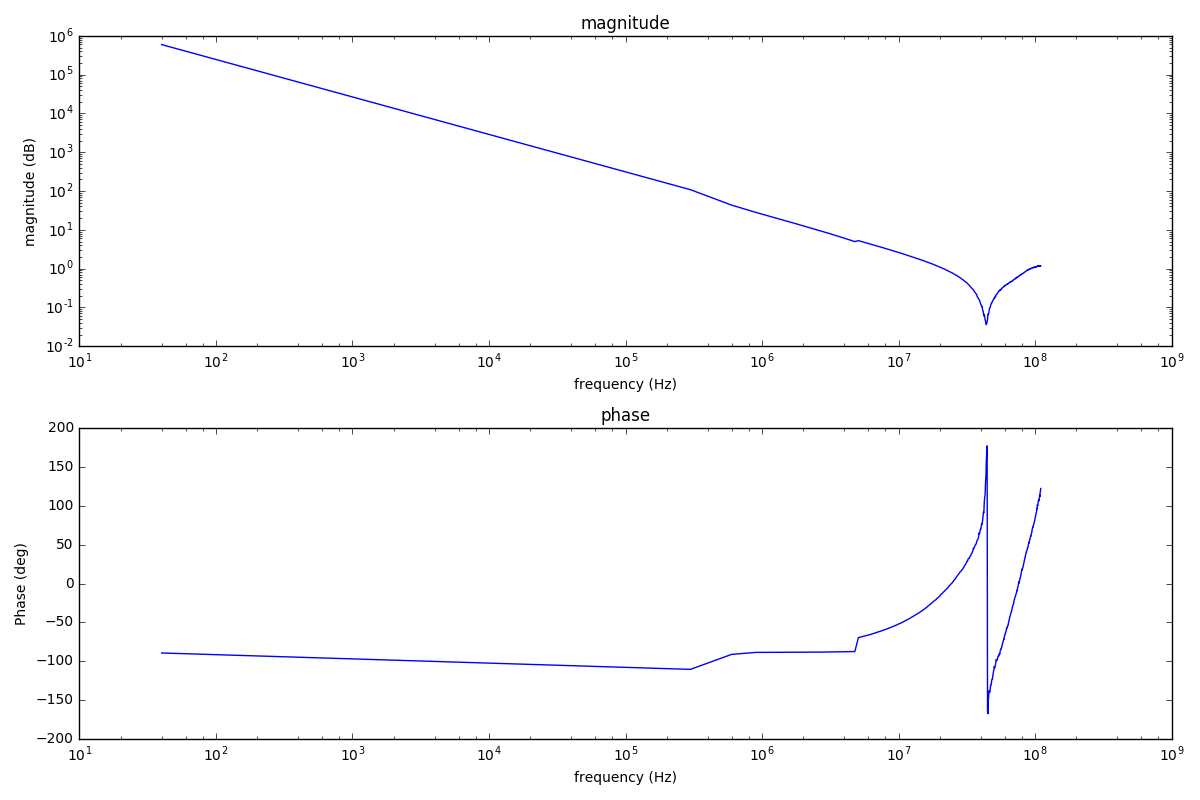
\includegraphics[width=0.3\textwidth]{src/1/figures/capa_hf_response.png}
  \caption{Frequency response of a 6.8nF capacitor}
  \label{fig:frequency-response-capa}
\end{figure}

Fig. \ref{fig:frequency-response-capa} displays the module versus frequency curve for a 6.8 nF CMS capacitor.
Until 45 MHz, the capacitor exhibits a perfect behavior.
At this resonant frequency it behaves as a very low-valued resistor (also called Equivalent Series Resistor or ESR), which is the series resistance in the HF model.
Over 45 MHz, the capacitor behaves as an inductor.
The slope of the curve before 45 MHz is determined by the capacitor value and is given by C\textomega{} or 2\textomega{}Cf.
It shows a phase of -90 degrees.
After 45 MHz, it is determined by the parasitic inductor value and given by -L\textomega{} or -2\textomega{}Lf, with a phase of +90 degrees.
With these two formulas, values for parasitic inductor and capacitor can be computed very easily from a measurement.
Once done, the parasitic resistor value is simply the module’s value (converted to ohms from dB) at the resonant frequency.

The same method applies for a real inductor or resistor.
In the case of capacitors, for a given package, first observations tend to show few variations for the parasitic inductance, even with capacitors of different values.
Thus the parasitic inductance seems mostly related to the package, with values between 1nH and 5nH.
This is especially true for CMS packages.
If confirmed, this observation means that there is no need to characterize every single passive device, but instead it is possible to take a parasitic model corresponding to the package.

% Non-linear high power behavior
%TODO: Find articles that show non-linear behavior
The other point to consider is variations of the main nominal rating of the passive device when exposed to significantly high levels of injection. Multi-layers ceramic capacitors (MLCC) seem mostly concerned about this phenomenon \cite{capa-esd-cz}, where the capacitance decreases at high voltages.
Not happening with X7R capacitors ?

\subsection{Other devices}
%TODO: Diodes ?
%TODO: Common mode choke ?
% etc

\subsection{Propagation phenomena}

%TODO
Sometimes important to take into account for the modelling and assembling of models

Propagation and reflection are the two main phenomena occurring at the nanosecond timescale that are ignored in standard time-domain electrical simulations.

Propagation is a phenomenon that always occurs but is negligible over a few tens microseconds.
Below that timescale it must be taken into account because it has a major impact on the waveforms.
This is due to the fact that observation times are in the same range than electrical wave propagation times.

Reflection happens when an electrical wave propagates and reaches a point where two propagation media are mismatched (two coaxial cables of different characteristic impedance for example).

These two effects and in combination can impact waveform in some specific scenario

% Measurement artifact
Spike visible on measurements but is just an artifact
Caused by a delay between an intended measurement point and where the measurement is actually performed
Delay because of a cable for instance
Setup given in Fig \ref{fig:setup-measurement-spike}

\begin{figure}[!h]
  \centering
  \includegraphics[width=0.3\textwidth]{src/1/figures/setup_measurement_spike.pdf}
  \caption{Typical setup causing a measurement artifact}
  \label{fig:setup-measurement-spike}
\end{figure}

The process that generates this measurement glitch starts with the injection of a fast rectangular pulse.
The pulse propagates towards point A (step 1).

\begin{figure}[!h]
  \centering
  \includegraphics[width=0.3\textwidth]{src/1/figures/spike_generation_1.pdf}
  \caption{Spike generation - step 1}
  \label{fig:spike-step-1}
\end{figure}

At the moment it reaches A, the capacitor load is not immediately visible.
It is “hidden” from point A by the short delay.
Thus, the voltage rises, depending at this point only on the characteristic impedances of the cables.
A part of the pulse propagates towards the load and a part toward Vout (depending on the impedance ratio) (step 2).

\begin{figure}[!h]
  \centering
  \includegraphics[width=0.3\textwidth]{src/1/figures/spike_generation_2.pdf}
  \caption{Spike generation - step 2}
  \label{fig:spike-step-2}
\end{figure}

The impulse reaches then the load (step 3), and propagates back toward A, settling the voltage at A to
V – (V – Vload) = Vload (forward travelling wave minus reflected wave from load) (step 3).
The capacitor is supposed to be charging at constant current, voltage rises following a linear curve.

\begin{figure}[!h]
  \centering
  \includegraphics[width=0.3\textwidth]{src/1/figures/spike_generation_3.pdf}
  \caption{Spike generation - step 3}
  \label{fig:spike-step-3}
\end{figure}

Now the voltage at point A is defined by the load.
However before that, the voltage rose and generated a peak that will hit Vout after a delay.
This peak preceding the capacitor charge is detailed on figure \ref{fig:spike-step-4}.
The amplitude is exaggerated for illustration purposes

\begin{figure}[!h]
  \centering
  \includegraphics[width=0.3\textwidth]{src/1/figures/spike_generation_4.pdf}
  \caption{Spike generation - step 4}
  \label{fig:spike-step-4}
\end{figure}

In a more realistic situation, if the short delay is of the same order of magnitude than the pulse risetime, the generated peak will be a non-negligible fraction of the initial pulse amplitude.

\begin{figure}[!h]
  \centering
  \includegraphics[width=0.3\textwidth]{src/1/figures/spike_generation_5.pdf}
  \caption{Measured waveform}
  \label{fig:spike-step-4}
\end{figure}

% Unterminated cables
Because of propagation and reflection phenomena, elements that are normally ignored in standard simulations can no longer be neglected.
A perfect illustration of this point are cables connected to the circuit on one end, and left floating on the other end (or in high impedance)
In regular simulations, they can removed entirely.
With ESD simulations, they will induce oscillations and amplitude changes

\begin{figure}[!h]
  \centering
  \includegraphics[width=0.3\textwidth]{src/1/figures/setup_unconnected_cable.pdf}
  \caption{Typical setup causing oscillations}
  \label{fig:setup-unconnected-cable}
\end{figure}

%TODO: Rewrite completely
Transient current propagates toward the unconnected end
Reflects entirely at the high impedance termination
Comes back inside the circuit, absorbing a part of the initial current and supplying it later on.
The consequence is an undershoot followed by a delayed overshoot (fig. 15).
%TODO: Put a waveform ?

\gls{tlp} is a perfect example of an application exploiting an unterminated cable

% Feeding cables
%TODO: Talk about location of measurement point
Similarly, all cables on the propagation path (Fig. \ref{fig:setup-feeding-cable}) must not be neglected just because they are matched with the circuit.
The delay they introduce impacts greatly the waveforms.
TLP generators always require a cable to connect the load under test to the generator.
This connection cable plays a role in the final waveform.
In simulation, if omitted, the waveform is very rectangular and clean (Fig. \ref{fig:comparison-feeding-cable}).
When the cable is added, the presence of reflections with this delay changes quite a lot the waveform that now has an initial step between 00 and XX ns, with an amplitude corresponding to the TLP charging voltage and not the circuit operating point
XX ns corresponds exactly to (twice ?) the delay of the feeding coaxial cable.

\begin{figure}[!h]
  \centering
  \includegraphics[width=0.3\textwidth]{src/1/figures/setup_feeding_cable.pdf}
  \caption{Minimal TLP generator with feeding cable and a mismatched load}
  \label{fig:setup-feeding-cable}
\end{figure}

\begin{figure}[!h]
  \centering
  \includegraphics[width=0.3\textwidth]{src/1/figures/comparison_feeding_cable.png}
  \caption{Simulated waveform with and without feeding cable}
  \label{fig:comparison-feeding-cable}
\end{figure}

% Conclusion
%TODO: Detail
Beyond these particular examples, the idea is to be cautious about even short delays when assembling models from the library.
